\documentclass[border=6pt]{standalone}
% Redrawn after Figure 1 of Vaswani et al., "Attention Is All You Need", NeurIPS 2017.

% --- packages (mirror these in meta.json "requires") ---
\usepackage[T1]{fontenc}
\usepackage{helvet}
\renewcommand{\familydefault}{\sfdefault}
\usepackage{tikz}
\usetikzlibrary{arrows.meta}

% --- colors sampled from the original figure ---
\definecolor{tfattention}{HTML}{FFE2BB}
\definecolor{tfnorm}{HTML}{F0F3BD}
\definecolor{tffeedforward}{HTML}{C2E8F7}
\definecolor{tfembedding}{HTML}{FCE0E1}
\definecolor{tflinear}{HTML}{DBDFEF}
\definecolor{tfsoftmax}{HTML}{CCE7CF}
\definecolor{tfstack}{HTML}{F3F3F4}

% ==== parameters (edit these) ============================================
\def\gridunit{0.014}   % size of one layout unit (cm); scales the whole drawing
\def\linew{1.35pt}     % weight of every box and arrow
% labels
\def\attentionlabel{Multi-Head\\Attention}
\def\maskedlabel{Masked\\Multi-Head\\Attention}
\def\normlabel{Add \& Norm}
\def\feedforwardlabel{Feed\\Forward}
\def\inputembedlabel{Input\\Embedding}
\def\outputembedlabel{Output\\Embedding}
\def\poslabel{Positional\\Encoding}
\def\inputslabel{Inputs}
\def\outputslabel{Outputs\\(shifted right)}
\def\linearlabel{Linear}
\def\softmaxlabel{Softmax}
\def\probslabel{Output\\Probabilities}
\def\repeatlabel{N$\times$}
% =========================================================================

\begin{document}
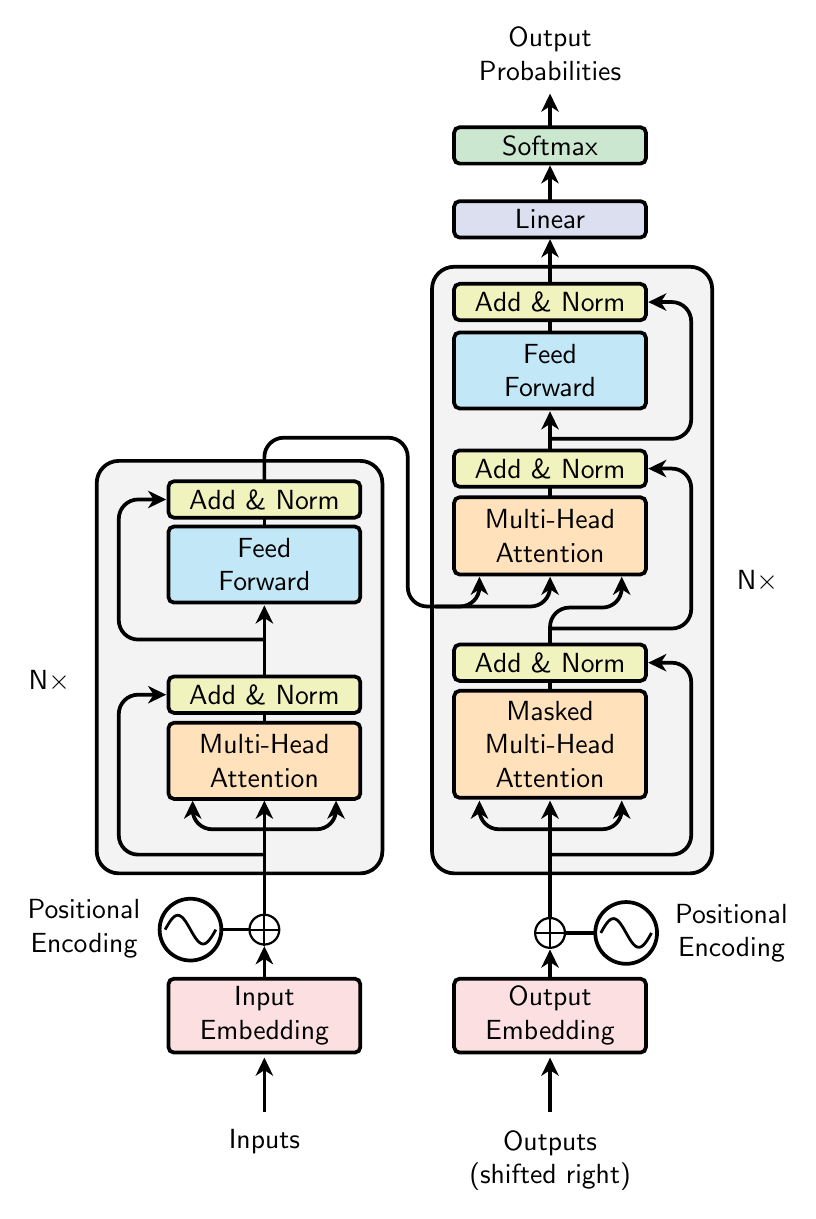
\begin{tikzpicture}[
    x=\gridunit cm, y=-\gridunit cm,
    >={Stealth[length=2.3mm, width=2.2mm, inset=0.7mm]},
    font=\normalsize,
    wire/.style={draw=black, line width=\linew, rounded corners=7pt},
    flow/.style={wire, ->},
    layer/.style={
      draw=black, line width=\linew, rounded corners=2pt, align=center, inner sep=0pt,
      minimum width=174*\gridunit cm, minimum height=#1*\gridunit cm,
    },
    stack/.style={draw=black, line width=\linew, fill=tfstack, rounded corners=8pt},
    caption/.style={align=center, inner sep=0pt},
    addop/.style={circle, draw=black, fill=white, line width=0.8pt, inner sep=0pt, minimum size=27*\gridunit cm},
    wave/.style={circle, draw=black, fill=white, line width=\linew, inner sep=0pt, minimum size=56*\gridunit cm},
  ]
  \newcommand{\addsymbol}[1]{
    \draw[line width=0.7pt] (#1.north) -- (#1.south);
    \draw[line width=0.7pt] (#1.west) -- (#1.east);
  }
  \newcommand{\sinewave}[2]{
    \draw[line width=1pt, smooth] plot[domain=-1:1, samples=40] ({#1+23*\x},{#2+13*sin(180*\x)});
  }

  % --- the two repeated stacks ---
  \draw[stack] (98,418) rectangle (357,792);
  \draw[stack] (402,242) rectangle (656,792);
  \node[caption] at (55,618) {\repeatlabel};
  \node[caption] at (697,527) {\repeatlabel};

  % --- encoder wiring, bottom to top ---
  \node[caption] (inputs) at (250,1035) {\inputslabel};
  \draw[flow] (250,1008) -- (250,959);
  \draw[flow] (250,888) -- (250,858);
  \draw[flow] (250,829) -- (250,726);
  \draw[flow] (250,752) -- (185,752) -- (185,726);
  \draw[flow] (250,752) -- (315,752) -- (315,726);
  \draw[flow] (250,775) -- (118,775) -- (118,630) -- (161,630);
  \draw[wire] (250,655) -- (250,646);
  \draw[flow] (250,613) -- (250,549);
  \draw[flow] (250,580) -- (118,580) -- (118,453) -- (161,453);
  \draw[wire] (250,478) -- (250,469);

  % --- encoder memory enters the decoder's middle attention ---
  \draw[flow] (250,436) -- (250,397) -- (380,397) -- (380,550) -- (509,550) -- (509,523);
  \draw[flow] (405,550) -- (445,550) -- (445,523);

  % --- decoder wiring, bottom to top ---
  \node[caption] (outputs) at (509,1053) {\outputslabel};
  \draw[flow] (509,1008) -- (509,959);
  \draw[flow] (509,888) -- (509,861);
  \draw[flow] (509,832) -- (509,726);
  \draw[flow] (509,752) -- (445,752) -- (445,726);
  \draw[flow] (509,752) -- (574,752) -- (574,726);
  \draw[flow] (509,775) -- (637,775) -- (637,601) -- (598,601);
  \draw[wire] (509,627) -- (509,616);
  \draw[flow] (509,585) -- (509,551) -- (574,551) -- (574,523);
  \draw[flow] (509,570) -- (637,570) -- (637,425) -- (598,425);
  \draw[wire] (509,451) -- (509,441);
  \draw[flow] (509,409) -- (509,373);
  \draw[flow] (509,398) -- (637,398) -- (637,274) -- (598,274);
  \draw[wire] (509,302) -- (509,290);
  \draw[flow] (509,259) -- (509,217);
  \draw[flow] (509,183) -- (509,150);
  \draw[flow] (509,116) -- (509,85);

  % --- encoder layers ---
  \node[layer=67, fill=tfembedding] (enc-embed) at (250,921) {\inputembedlabel};
  \node[layer=69, fill=tfattention] (enc-attn) at (250,690) {\attentionlabel};
  \node[layer=33, fill=tfnorm] (enc-norm1) at (250,630) {\normlabel};
  \node[layer=69, fill=tffeedforward] (enc-ff) at (250,512) {\feedforwardlabel};
  \node[layer=33, fill=tfnorm] (enc-norm2) at (250,453) {\normlabel};

  % --- decoder layers ---
  \node[layer=67, fill=tfembedding] (dec-embed) at (509,921) {\outputembedlabel};
  \node[layer=97, fill=tfattention] (dec-masked) at (509,675) {\maskedlabel};
  \node[layer=33, fill=tfnorm] (dec-norm1) at (509,601) {\normlabel};
  \node[layer=70, fill=tfattention] (dec-attn) at (509,486) {\attentionlabel};
  \node[layer=33, fill=tfnorm] (dec-norm2) at (509,425) {\normlabel};
  \node[layer=69, fill=tffeedforward] (dec-ff) at (509,336) {\feedforwardlabel};
  \node[layer=33, fill=tfnorm] (dec-norm3) at (509,274) {\normlabel};
  \node[layer=33, fill=tflinear] (linear) at (509,199) {\linearlabel};
  \node[layer=33, fill=tfsoftmax] (softmax) at (509,132) {\softmaxlabel};
  \node[caption] (probs) at (509,49) {\probslabel};

  % --- positional encodings ---
  \draw[line width=\linew] (212,843) -- (236,843);
  \node[wave] (enc-wave) at (183,843) {};
  \sinewave{183}{843}
  \node[addop] (enc-plus) at (250,843) {};
  \addsymbol{enc-plus}
  \node[caption, anchor=east] at (138,842) {\poslabel};

  \draw[line width=\linew] (523,846) -- (549,846);
  \node[wave] (dec-wave) at (578,846) {};
  \sinewave{578}{846}
  \node[addop] (dec-plus) at (509,846) {};
  \addsymbol{dec-plus}
  \node[caption, anchor=west] at (622,846) {\poslabel};

\end{tikzpicture}
\end{document}
